%!TEX root = depicto-top.tex
%%%%%%%%%%%%%%%%%%%%%%%%%%%%%%%%%%%%%%%%%%%%%%%%%%%%%%%%%%%%%%%%%%%%%%%%%%%%%%
%% Background
%%%%%%%%%%%%%%%%%%%%%%%%%%%%%%%%%%%%%%%%%%%%%%%%%%%%%%%%%%%%%%%%%%%%%%%%%%%%%%

\chapter{Resources}
\label{chap:Background}

This chapter provides background to the third-party resources upon which the
\depicto\ system draws. First up is the extensive, open-source pictographic
symbol set \sclera. Here, the discussion centers on a semantic inventory of the
symbol set which later forms the basis for the \depicto\ system's approach to
\sclera\ as a (simple) language whose grammar can be \emph{modelled} formally.
The theoretical framework within which this modelling process is carried out,
viz., Head-driven Phrase Structure Grammar (\hpsg, \citet{pollard1994head}), is
introduced next, along with the precise formalisms, frameworks, resources, and
tools used in the development and operationalisation of the computationally
implemented grammars that form the \depicto\ system's analysis and generation
modules. Barring the \hpsg\ framework itself, these resources have all been
developed within the \delphin\
community\footnote{http://www.delph-in.net/wiki/index.php/Home} (an informal
international umbrella organisation for grammar engineering research that takes
the \hpsg\ framework as its starting point), and they are freely available on
the \delphin\ public repository. In a separate third section, the \logon\
system for semantic transfer between monolingual \delphin\ grammars is
introduced. Similarly developed within \delphin, this system, which allows
grammars to `communicate' with one another (albeit it in a one-directional
way), forms the keystone to the \depicto\ pipeline and provides a mechanism
that ensures the modularity of the system as a whole.

\section{The \sclera\ symbol set}
\label{sec:sclera}

In the \depicto\ system, input sequences are composed using pictographic
symbols taken from a subset of the extensive and freely available \sclera\
symbot set. In its entirety, \sclera\ comprises upwards of 13,000 pictographs
that have been specifically designed to meet the communicative needs of people
with ID. Visually, these symbols are characterized by a large degree of
uniformity, with most adhering to a strict black-and-white color scheme. While
several alternatives to \sclera\ exist (some of which are mentioned further
down), none lend themselves quite so well to the desire for expressivity, as
well as the open-source mentality, that has guided the development of the
system presented in this thesis. Moreover, \sclera\ is the pictographic
language of choice in a number of homegrown AAC technologies, including the
Text2Picto system and the Picto2Text system (the latter already discussed in
section~\ref{sub:picto2text}). The remainder of this section briefly discusses
the background and aims of the \sclera\ project, gives a brief overview of the
kinds of pictographs found in the symbol set, discusses the Sclera2Cornetto
resource for pictograph-WordNet linking, and lists a number of alternative
options, with particular attention to the \emph{Beta} language.

\subsection{Bottom-up development} % project background

The vast size of the \sclera\ set as it stands today is by all accounts a
testament to the success of one of the main aims of the \sclera\ NPO. As set
out in its mission statement \citep{sclera2011voorstelling}, this is to provide
various social target groups, particularly people with cognitive disabilities,
with accessible and affordable (in this case: free) visual aids that are
tailored to the needs of individual users. In addition to designing and
distributing pictographs, the \sclera\ group also provides users and caretakers
with free advice on how to use them. Through these interactions, as well as via
the \sclera\ website \footnote{http://www.sclera.be/en/vzw/home}, the
developers have received an increasing number of requests for new and specific
pictographs to which they have been happy to respond. Thus, since the release
of the first registered batch of pictographs in 2007, the \sclera\ set has
grown from 200 to just over 13,000 pictographs \citep{vandeghinste2014linking}.

However, size is not the only aspect that the \sclera\ group's bottom-up
approach to pictograph development has influenced. In fact, the very function
of the pictographs themselves has changed: while originally they were intended
as a way of communicating instructions \emph{to}, they now also address the
communicative needs of the users. In terms of design aesthetics, the bottom-up
approach was influential in the adoption of the black-and-white color scheme.
Its uniformity was found to lend the images a sense of `calmness' and proved to
be very popular among people with autism, and the higher contrast appealed to
people with partial visual impairments. Finally, user feedback suggested that
certain groups vary in their preference for a particular depiction of a
concept, finding one pictograph more obvious than others. In the \sclera\ set,
therefore, concepts can stand in a one-to-many relationship with pictographs,
as \cref{fig:differentdogs} shows for the concept `dog'.

\begin{figure}[h]
    \centering
    % \vspace{1cm}
    \begin{subfigure}{0.22\textwidth}
        
\includegraphics[width=0.85\linewidth]{sclera/hond1}
        % \caption{...}
    \end{subfigure}
    \begin{subfigure}{0.22\textwidth}
        
\includegraphics[width=0.85\linewidth]{sclera/hond2}
        % \caption{...}
    \end{subfigure}
    \begin{subfigure}{0.22\textwidth}
        
\includegraphics[width=0.85\linewidth]{sclera/hond3}
        % \caption{...}
    \end{subfigure}
    \begin{subfigure}{0.22\textwidth}
        
\includegraphics[width=0.85\linewidth]{sclera/hond4}
        % \caption{...}
    \end{subfigure}
    \caption{Different \sclera\ depictions of the concept `dog'}
    \label{fig:differentdogs}
\end{figure}

\subsection{Taking inventory} % inventory
\label{sub:scleraInventory}

The \sclera\ set is primarily composed of pictographs depicting entities or
processes. In terms of function, these correspond to nouns and verbs. Within
the `nominal' category, pictographs generally do not distinguish between
singular and plural readings, nor do they encode quantification or reference,
since quantifiers and determiners do not exist in the \sclera\ language. (The
exception concerns a small set of pictographs that convey `pronominal' meaning,
including pictographic equivalents of personal, demonstrative, possessive, and
interrogative pronouns.) As a result of the customization-ready approach
discussed above, there is room for hyponymy, with specific realizations of a
particular concept receiving their own pictographic depiction, as
\cref{fig:bikes} shows for a sample of different realizations of the hypernym
`bicycle'. Next, within the verbal category, pictographs are similarly
underspecified for number, as well as tense and, unsurprisingly, inflection.
Auxiliary verbs are absent, although there does exist a pictographic
representation for the copular verb `be'. A small set of adjectives is also
included. Most of these relate to emotion.

\begin{figure}[h]
    \centering
    % \vspace{1cm}
    \begin{subfigure}{0.22\textwidth}
        \includegraphics[width=0.85\linewidth]{{"sclera/fiets zijwieltjes"}}
        % \caption{...}
    \end{subfigure}
    \begin{subfigure}{0.22\textwidth}
        
\includegraphics[width=0.85\linewidth]{sclera/fiets}
        % \caption{...}
    \end{subfigure}
    \begin{subfigure}{0.22\textwidth}
        \includegraphics[width=0.85\linewidth]{{"sclera/rolstoel fiets"}}
        % \caption{...}
    \end{subfigure}
    \begin{subfigure}{0.22\textwidth}
        
\includegraphics[width=0.85\linewidth]{{sclera/tandem}}
        % \caption{...}
    \end{subfigure}
    \caption{Different kinds of bikes}
    \label{fig:bikes}
\end{figure}

In addition to pictographs that depict simple concepts, most of these
corresponding to a single word in some natural language (depending on the
language, of course), a sizeable portion of the \sclera\ inventory consists of
pictographs that represent conceptual complexes. For pictographs depicting
entities this amounts to a form of nominal compounding. Within the verbal
category, it is not uncommon for a verbal head and one or more of its
complements to be rolled into a single pictograph. These complex pictographs
provide a mechanism for expressing relations which, in English and Dutch, are
generally conveyed by prepositions (another category missing from the content
word-oriented symbol set). Adverbial relations, which also do not appear in the
system set, can similarly be expressed.

\begin{figure}[h]
    \centering
    % \vspace{1cm}
    \begin{subfigure}{0.22\textwidth}
        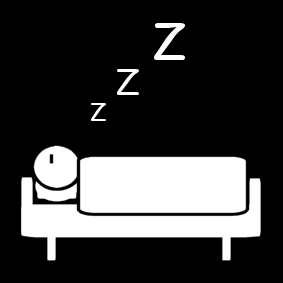
\includegraphics[width=0.85\linewidth]{{sclera/slapen}}
        \caption{`sleep'}
    \end{subfigure}
    \begin{subfigure}{0.22\textwidth}
        
\includegraphics[width=0.85\linewidth]{sclera/dansen}
        \caption{`dance'}
    \end{subfigure}
    \begin{subfigure}{0.22\textwidth}
        
\includegraphics[width=0.85\linewidth]{{sclera/geven}}
        \caption{`give'}
    \end{subfigure}
    \begin{subfigure}{0.22\textwidth}
        
\includegraphics[width=0.85\linewidth]{sclera/koken}
        \caption{`cook'}
    \end{subfigure}
    \caption{Simplex situations ('verbs' pictos)}
    \label{ex:sclera:simplex-situations}
\end{figure}

\begin{figure}[h]
    % \label{differentdogs}
    \centering
    \begin{subfigure}[t]{0.22\textwidth}
        
\includegraphics[width=0.85\linewidth]{{sclera/muziek-luisteren}}
        \caption{`listen' + `music'}
    \end{subfigure}
    \begin{subfigure}[t]{0.22\textwidth}
        
\includegraphics[width=0.85\linewidth]{sclera/toilet-gaan}
        \caption{`go (to)' + `bathroom'}
    \end{subfigure}
    \begin{subfigure}[t]{0.22\textwidth}
        
\includegraphics[width=0.85\linewidth]{sclera/koken-ik}
        \caption{`I' + `cook'}
    \end{subfigure}
    \begin{subfigure}[t]{0.22\textwidth}
        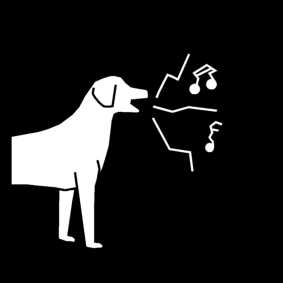
\includegraphics[width=0.85\linewidth]{sclera/hond-blaffen}
        \caption{`dog' + `bark'}
    \end{subfigure}
    \caption{Complex situations}
\end{figure}

\begin{figure}[h]
    % \label{}
    \centering
    \begin{subfigure}[t]{0.22\textwidth}
        \includegraphics[width=0.85\linewidth]{{"sclera/hij"}}
        \caption{`he/him'}
    \end{subfigure}
    \begin{subfigure}[t]{0.22\textwidth}
        \includegraphics[width=0.85\linewidth]{{"sclera/jij"}}
        \caption{`you (singular)'}
    \end{subfigure}
    \begin{subfigure}[t]{0.22\textwidth}
        \includegraphics[width=0.85\linewidth]{{"sclera/jullie"}}
        \caption{`you (plural)'}
    \end{subfigure}
    \begin{subfigure}[t]{0.22\textwidth}
        \includegraphics[width=0.85\linewidth]{{"sclera/spel mijn beurt"}}
        \caption{`mine'}
    \end{subfigure}
    \caption{`Pronominal' pictographs}
    \label{}
\end{figure}

\begin{figure}[h]
    % \label{}
    \centering
    \begin{subfigure}[t]{0.22\textwidth}
        \includegraphics[width=0.85\linewidth]{{"sclera/peper en zout"}}
        \caption{`salt and pepper'}
    \end{subfigure}
    \begin{subfigure}[t]{0.22\textwidth}
        \includegraphics[width=0.85\linewidth]{{"sclera/eten en drinken"}}
        \caption{`food and drink'}
    \end{subfigure}
    \begin{subfigure}[t]{0.22\textwidth}
        \includegraphics[width=0.85\linewidth]{{"sclera/baby zeep"}}
        \caption{`baby soap'}
    \end{subfigure}
    \caption{Complex entities (nominal compounds)}
    \label{}
\end{figure}

\begin{figure}[h]
    % \label{}
    \centering
    \begin{subfigure}[t]{0.22\textwidth}
        \includegraphics[width=0.85\linewidth]{{"sclera/jaloers boos"}}
        \caption{`jealous'}
    \end{subfigure}
    \begin{subfigure}[t]{0.22\textwidth}
        \includegraphics[width=0.85\linewidth]{{"sclera/blij"}}
        \caption{`happy'}
    \end{subfigure}
    \begin{subfigure}[t]{0.22\textwidth}
        \includegraphics[width=0.85\linewidth]{{"sclera/bed niet goed liggen 2"}}
        \caption{`bed uncomfortable'}
    \end{subfigure}
    \caption{Emotion/attitude}
    \label{}
\end{figure}

\begin{figure}[h]
    \centering
    \scriptsize
    \begin{subfigure}[t]{0.22\textwidth}
        \includegraphics[width=0.85\linewidth]{{"sclera/asbak 4 kruis rood"}}
        \caption{`no smoking' (red cross)}
    \end{subfigure}
    \begin{subfigure}[t]{0.22\textwidth}
        \includegraphics[width=0.85\linewidth]{{"sclera/aanraken ander kruis rood"}}
        \caption{`no touching others' (red cross)}
    \end{subfigure}
    \begin{subfigure}[t]{0.22\textwidth}
        \includegraphics[width=0.85\linewidth]{{"sclera/delen snoep groen"}}
        \caption{`share candy' (green)}
    \end{subfigure}
    \begin{subfigure}[t]{0.22\textwidth}
        \includegraphics[width=0.85\linewidth]{{"sclera/veiligheidsgordel zelf aandoen groen"}}
        \caption{`buckle seatbelt'  (green)}
    \end{subfigure}
    \caption{`Imperative' pictographs (directives)}
    \label{}
\end{figure}

\begin{figure}[h]
    % \label{}
    \centering
    \begin{subfigure}[t]{0.22\textwidth}
        \includegraphics[width=0.85\linewidth]{{"sclera/gelijke kansen"}}
        \caption{`equal opportunities'}
    \end{subfigure}
    \begin{subfigure}[t]{0.22\textwidth}
        \includegraphics[width=0.85\linewidth]{{"sclera/herhalen"}}
        \caption{`repeat'}
    \end{subfigure}
    \caption{Abstract concepts}
    \label{}
\end{figure}


Finally, the \sclera\ set includes a number of pictographs which are slightly
more marked. A first subset comprises opposition pairs. These often relate to
behaviour. In contrast to the rest of symbol set (with a few exceptions), these
pictographs make use of color: their (black) background is swapped out for
either a green or red one to indicate permission or prohibition, respectively.
Other pictographs, most of them `verbal', are marked for `positive' or
`negative' connotation on top of the concept that they depict, allowing the
user to express his attitude toward, for example, a situation of `saying
goodbye'. On a thematic level, the \sclera\ set contains a wide variety of
pictographs relating to independent living (bank cards, ATMs, taking the train,
etc.), culture, contemporary lifestyle and technology (electronic
communication, drugs, music), as well a number of `taboo' subjects such as
sexuality, religion, hygiene, and death.

\subsection{Choosing \sclera}
\label{sub:Beta}

\sclera\ is already used by the Picto2Text system \citep{sevens2015natural}, as
well as by its forerunner, the Text2Picto system
\citep{vandeghinste2015translating}, both introduced in
section~\ref{sub:picto2text}. As is discussed there, both translation systems
rely on previously established links between pictograph identifiers on the one
hand and WordNet synsets on the other \citep{vandeghinste2014linking}. (These
synsets are in turn linked to the EuroWordNet grid and SUMO ontology.) In order
to keep open the option of integration with the Picto2Text system further down
the road, as well as to enjoy the possible future benefits of the rich
lexical-semantic resource upon which its operation relies, the \depicto\ system
follows the Picto2Text example and adopts the \sclera\ set.

There are alternatives, however. Filtering these on availability (the operative
criterion being `free'), expressiveness, and success in user testing, the next
best option is the \emph{Beta} symbol set. The pictographs in this set make
much more use of color than those in \sclera, which, despite the resulting lack
of uniformity, makes them visually more appealing for some people. Aesthetics
aside, there are some important differences with the \sclera\ set. For one
thing, \emph{Beta} symbols depict only simplex concepts, as opposed to allowing
compounding and complexing. For another, prepositional relations are depicted.
While the first divergence makes little difference for compatibility with a
\sclera-oriented system, as \emph{Beta} can simply be treated as a subset of
the expressive scope of \sclera, the second difference makes things a little
trickier, since prepositional pictographs are not supported by the grammar of
\sclera\ which the \depicto\ system uses. For the time being, therefore,
\emph{Beta} is left to the side, although it is important to realize that it is
there, if only because it \emph{is} supported by the Picto2Text and Text2Picto
systems.

%-----------------------------------------------------------------------------
\section{Grammar engineering: The \delphin\ toolkit}
\label{sec:delph-in}

There are numerous grammar formalisms for which parsing and (slightly less
often) generation implementations exist. These include -- to name a few --
Context-Free Grammars (CFGs; \citet{chomsky1959certain}, Unification Grammars
(UGs; i.a. \citet{shieber1983formalism}), (Lexicalized) Tree-Adjoining Grammars
((L)TAGS; \citet{joshi1997tree}), and Dependency Grammars (DGs;
\citet{vater1975toward}). With the exception perhaps of traditional CFGs, each
of these formalisms has its merits. Additionally, their implementations vary in
the algorithms that they use, the degree to which these algorithms are
optimized, and the extent to which they have been designed with a
particular theoretical framework for syntactic analysis in mind. In short,
choosing a formalism is no easy task.

To keep things simple, therefore, both the analysis and generation modules
found in the \depicto\ system make use of the same unification-based formalism,
are written within the same framework, viz., \hpsg\ \citep{pollard1994head},
and rely on the same software for processing. These resources, each
representing multiple person-years of work, are all developed and distributed
by the same community: the \emph{Deep Linguistic Processing with HPSG
Initiative} (\delphin \footnote{http://moin.delph-in.net/}), an international
collaborative grammar engineering effort aimed at developing open-source NLP
tools for `deep' linguistic processing of human language. These tools can be
augmented with statistical processing methods, but the basis is thoroughly
symbolic. Through collaboration, with founding members coming from Stanford's
CSLI (USA), from Germany's DKFI and University of Saarland, and from Norway's
University of Science \& Technology and University of Oslo, the \delphin\
project has made it significantly more cost-effective to develop efficient
large-scale implemented grammars. It has also made the development process a
great deal more rewarding by providing a variety of specialized tools to
process grammars with, the most important relating to parsing, generation and,
as we shall see in the next section, the transfer of semantic representations
for translation and paraphrasing purposes. Some of these tools are intended for
production, and \delphin\ grammars and tools are already in place in a number
of commercial applications.

The intercompatibility of \delphin\ tools and \delphin\ grammars, even though
these are often developed independently of another, is due to the convergence
on a small set of common descriptive formalisms. The first such reference
formalism relates to the specific variant of typed feature structure logic
which all \delphin\ grammars are expected to follow. (Typed feature structures
form the primary data structure in \hpsg\ as well as the LFG and CG frameworks,
both of which, incidentally, are also compatible with the \delphin\ grammar
processors.) A second reference formalism is the Minimal Recursion Semantics
format for semantic representation, which generally forms the main output of a
\delphin\ parser, and from which \delphin\ grammars are able to generate. Both
these formalisms, as well as the declarative language used to implement them,
will be discussed in more detail in the course of the current section.

The following provides a brief introduction to the \hpsg\ framework, discusses
the \delphin-style typed feature structure (TFS) formalism in more detail, and
takes a look at the declarative specification language in which grammar files
are written (\tdl) as well as the way in which individual files combine to form
a complete HPSG grammar. After introducing the \mrs\ formalism for semantic
representation next, we turn to the \lingo\ Grammar Matrix starter-kit, which
provides the `core' for the grammars used by the \depicto\ system's analysis
and generation modules. Finally, the relatively recent \ace\ system is
introduced, an all-in-one \delphin\ grammar processor designed for speed and
efficiency, with support for transfer-based machine translation.

\subsection{Computationally implemented HPSG}
\label{sub:HPSG}

This subsection presents a lightning introduction to the framework of
Head-driven Phrase Structure Grammar (\hpsg) \citep{pollard1994head} and
describes the specific typed feature structure formalism used in \delphin\
implementations. To round off, it looks at the expected source file structure
of a typical \delphin\ and details a selection of common differences between
theoretical and computational variants of \hpsg.

\subsubsection{The basic theoretical framework} % or the formalism?

Head-driven Phrase Structure Grammar (\hpsg) is a strongly lexicalist, modular,
unification-based linguistic theory originally developed by Ivan Sag and Carl
Pollard in the mid-1980s \citep{pollard1994head}. Unlike transformational
grammars, it is entirely surface-oriented, and treats linguistic objects not as
trees, but as structured sets of constraints that can be modelled by means of
\emph{feature structures} (FSs) (informally: feature-value pairs; formally,
directed acyclic graphs). Within this model-theoretic approach, each linguistic
object, and thus each feature structure, is further seen as instantiating a
particular \emph{type}. The type to which a linguistic object belongs is
situated within a greater hierarchy of types. These are ordered from most
general to most specific according to the generality of the information, i.e.,
constraints, specified by the associated feature structure. This \emph{type
hierarchy} is used to capture both lexical and syntactic generalizations. The
constraining relation between types and their features is expressed by
\emph{typed feature structure descriptions}\footnote{The literature tends to
emphasize that there is a difference between these typed feature structure
descriptions and the typed feature structures (TFSs) which they describe
\citep{copestake2002implementing}. However, the difference is very subtle,
essentially boiling down to the fact that TFS descriptions place partial
constraints on possible models, whereas typed feature structures are understood
as maximally specific models that correspond to linguistic reality. Because of
this subtlety, particularly in an implementation-oriented context, where, prior
to compilation, grammars consist entirely of TFS \emph{descriptions}, I follow
\citet{copestake2002implementing}) in ignoring it except when it is absolutely
relevant.}, which are represented as attribute-value matrices (AVMs)
\citep{sag1999syntactic}.

To re-iterate the last paragraph slightly -- within the \hpsg\, framework all
linguistic objects are modelled as TFSs. On the linguistic level, the most
general type is that of the \emph{sign} (a tuple of phonological and
syntactic-semantic information) \citep{fokkens2014enhancing}, which has lexical
and phrasal signs as its subtypes. Lexical signs include lexemes and/or words.
Phrasal signs amount to the grammar rules that combine lexical or other
saturated phrasal TFSs (via the operation of unification) into larger
well-formed TFSs corresponding to immediate constituents. The principles that
determine both the syntactic and semantic well-formedness of these constituents
form an additional set of phrasal TFSs. As larger TFSs are built up (from a
parsing perspective), the phonological/orthographic information borne by
constituent TFS is appended, such that the root TFS, which is equivalent to the
root of a syntactic tree, contains the entire parsed string.

\begin{exe}[h]
    \ex\label{simpleTypeHierachy}Top of a typical \hpsg\ type hierarchy\\\\
    % 
\includegraphics[height=3cm]{placeholder}
    \begin{tikzpicture}[scale=0.9]
    \Tree [ .sign [
                    .{lexical sign}
                    word
                    lexeme
                  ]
                  [
                    .{phrasal sign}
                    {non-headed phrase}
                    {headed phrase}
                  ]
          ]
    \end{tikzpicture}
\end{exe}

True to its name, the \hpsg\ framework generally treats syntactic constituents
as consisting of a head structure and one or more sister structures which are
selected for by the head or, in some cases, select the head, but without
assuming its status. In terms of the valential relationship between the head
and non-head daughters of the mother node, the head-subject, head-complement,
head-specifier, and head-modifier rules are the most common, and most phrasal
rule types inherit from them. (Their names are sufficiently self-explanatory
for this purposefully brief introduction.) In order that the head of a
constituent is accessible to subsequent phrasal rules, its \textsc{head}
feature, which encodes syntactical features such as its part of speech, is
passed up by virtue of the Head Feature Principle \citep{sag2003syntactic},
which. The TFS through which this principle enters the grammar makes use of an
identity statement (notationally indicated with co-indexed variable tags) that
requires the value of the \textsc{head} feature of the mother TFS and the value
of the \textsc{head} feature of the head daughter TFS to be token-identical.
This mechanism of structure sharing is characteristic of \hpsg\, and, combined
with unification, accounts for much of its flexibility and elegance.

As a lexical theory, finally, \hpsg\ treats the lexicon as a rich and
structured object \citep{muller13hpsg-synopsis}. In order to avoid redundancy,
the type hierarchy includes a separate set of mostly unary lexical rules whose
`application' is constrained to TFSs of the type \emph{lexeme} and/or
\emph{word} (depending on the precise flavor of \hpsg\ one is working in).
These can be subdivided into inflecting/morphological/affixing rules and
non-inflecting/constant rules. While intuitively evident in theoretical
versions of \hpsg, the former, when implemented, requires additional machinery
which usually amounts to some form of regex substitution. Common examples of
usage cases for non-inflecting lexical rules include modification of the
valential requirements of a matrix verb in the passive voice and of a
ditransitive verb that can undergo `dative shift'. Unlike the rules discussed
above, lexical rules are less free as regards the order of their application,
particularly, as we shall see, when implemented, with inflecting rules always
coming before their inflecting counterparts (again, from the perspective of
parsing, that is).

%----------------------------------------------------------------------------

\subsubsection{The \delphin\ formalism of TFSs}
\label{ssub:delphin}

\delphin\ grammars consist of a specification of a type system and of various
typed feature structures (TFSs) which are to be inferred from this type system.
These TFSs, which function (among other) as grammar rules, lexical rules, and
lexical entries \citep{copestake2000appendix}, are considered well-formed on
the basis of a relatively conservative subset of the typed feature structure
logic described by \citet{carpenter1992logic}. This logic also forms the basis
of the machine-readable specification language in which \delphin\ grammars are
encoded: type-description language (\tdl) \citep{krieger1994tdl}. We will
return to \tdl\ shortly.

The selection of the \delphin\ formalism was guided by concerns about
linguistic adequacy grounded in \hpsg\ and about requirements for efficient
processing \citep{oepen2010disambiguate}. Informally, the formalism is
characterized as relating to a closed-world, multiple-inheritance type system
that enforces strong typing (i.e., every structure belongs to a type) and
strict appropriateness (i.e., all features a type can be defined for must be
introduced at some point in the inheritance hierarchy). At the same time, the
formalism allows types to be associated with arbitrarily complex constraints
(such as TFS embedding via structure sharing), which are inherited either upon
compilation or at runtime. The inheritance of constraints, moreover, is
monotonic, and features are introduced maximally, such that in instances of
multiple inheritance (which, to be clear, form the majority) from several
partial TFS descriptions, the result is always a unique most general structure,
i.e., a greatest lower bound. Compared to other variants of typed feature
structure logic, the \delphin\ formalism is very restricted. There is no room
for formal devices such as disjunction (which can lead to expensive
backtracking), negation, implication, inequality, default inheritance (this is
actually permitted, but rarely used), set-valued features and relational
constraints (e.g. `true' lists, which are implemented instead using the
mechanism of embedded feature-structures), and extensionality (anything that is
not in the grammar does not belong to the models which it can produce)
\citep{copestake2000appendix}. As a matter of fact, the only formal
device/operator which the \delphin\ TFS formalism uses is conjunction.

\paragraph{Type Description Language (\tdl)}
\label{par:tdl}

Set out in \citet{copestake2002implementing} (to date, still the best
introduction to \delphin-style grammar development), \tdl\ is the specification
language used to define types, their constraints, and their place in the type
hierarchy, i.e., in relation to their supertypes. \tdl\ descriptions always
have an AVM equivalent, as \cref{ex:avm-vs-tdl} shows for a non-linguistic
example. Feature structures are demarcated by opening and closing square
brackets. Feature names are conventionally written in uppercase, while their
values, which can be other types, are written in lowercase. If the value of a
feature is both a type \emph{and} and a more specific feature structure
appropriate to that type, then the two are separated by an ampersand (`\&') to
indicate conjunction/unification. Feature-value pairs are separated by commas,
and all \tdl\ descriptions must terminate in a period (`.'). Instead of using
boxed numbers, \tdl\ descriptions indicate structure sharing by means variable
names prefixed with a hashtag (or `octothorp', `pound sign', `\texttt{\#}').

\begin{exe}[h]
    \ex Equivalent AVM and \tdl\ descriptions for a (\textbf{non-linguistic}) typed feature structure
    \label{ex:avm-vs-tdl}
    \avmoptions{notactive}
    \small
    \begin{xlist}
        \ex AVM description\\\\
            % \scriptsize
            \begin{avm}
                \[ \asort{dog}
                   breed & \avmstring{Dalmation} \\
                   coat & \[ background & \@1 white \\
                             foreground & \[ \asort{spotted}
                                             SPOT-COLOR & black \] \] \\
                   fear & \avmstring{Cruela de Vil} \\
                   litter-size & more-than-100 \\
                   health-problems & \< \asort{deafness} \> \\
                   other & \[ favorite-camouflage-environment & \[ \asort{snow}
                                                         color & \@1 \] \] \]
            \end{avm}\\
            \vspace{0.5cm}
        \ex \tdl\ description
            \small
            \begin{verbatim}
dalmation := dog &
    [ BREED "dalmation",
      COAT [ BACKGROUND #camo-color & white,
             FOREGROUND spotted & [ SPOT-COLOR black ] ],
      FEAR  "Cruela de Vil",
      LITTER-SIZE more-than-100,
      HEALTH-PROBLEMS < deafness >,
      OTHER.FAVORITE-CAMOUFLAGE-ENVIRONMENT snow & [ COLOR #camo-color ] ].
            \end{verbatim}
    \end{xlist}
\end{exe}

\subsubsection{Components of a \delphin\ grammar}
\label{ssub:delphinstructure}

At the core of any \delphin\ grammar is its type hierarchy. This hierarchy can
be distributed over more than one \tdl\ file (e.g., for purposes of design,
debugging, clarity), but is interpreted by the grammar processor as building up
one large ontology of TFS descriptions.

The remaining components of the grammar are referred to as \emph{entries}. When
compiled or invoked by the processor, these give rise to maximally specific
typed feature structures. They comprise both rules and lexical entries. Once
again, these can be distributed over several \tdl\ files, but the processor
will interpret them accordingly. Phrasal rules are expanded upon compilation,
as are lexical rules, although these are treated separated so as to account for
the unique order-specific properties of the lexical rules, as well as the
intended behaviour of the phrasal rules, which, though specified as TFSs, are
interpreted as rewrite rules over other TFSs. Entries in the lexicon, finally,
are expanded at runtime rather than during compilation so as to keep down the
size of the compiled grammar. The configuration file associated with the
processor tells it how to interpret which components.

An small class of additional grammar entries is contributed by two files that
conventionally bear the names \texttt{roots.tdl} and \texttt{labels.tdl}.
\texttt{roots.tdl} contributes those TFSs that can function as start symbols in
the grammar, that is, as the root of a parse tree. \texttt{labels.tdl}
contributes the labels used to name the nodes in parse trees.

\subsubsection{Deviations from theoretical \hpsg}

While canonical theoretical \hpsg\ (which, for the sake of the discussion here,
I assume to be the flavor introduced in \citet{pollard1994head}) and
implemented \hpsg\ have, as one would expect, much in common, there are also
some differences in the analyses which they produce. These differences are relatively minor, but it helps to be aware of them nonetheless. The most salient, therefore, are briefly sketched out here.

\paragraph{Preference for unary or binary branching rules}
\label{par:naryvsbinary}

While the general phrasal rules, or `immediate dominance schemata'
\citep{pollard1994head}, of theoretical \hpsg\ generally license \emph{N-ary}
(viz., 1,2,3,4...n-ary) branching phrase structures \cref{ternary-branch}, such
rules are generally constrained to being either binary or unary in implemented
\hpsg. This is not to say that ternary, quaternary, etc. branching is ruled
out; it is simply dispreferred, as it leads to a significant increase in the
size of the search space that the parsing and generation algorithms need to
consider. The traditional analysis of the ditransitive valence schema of a verb
such as \emph{give} is instead analysed as two successive `applications' of
a binary head-complement rule, as in \cref{binary-branch}.

% uses qtree or tikz-qtree-compact
\begin{exe}
    \ex Ternary vs. binary branching analyses of ditransitive verb phrase (VP)\\
        \begin{xlist}
        \ex \label{ternary-branch} Ternary branching VP analysis\\
        \Tree [ .S
                     \qroof{the gorilla}.NP
                    [ .VP [ .V gave ]
                           \qroof{the scientist}.NP
                           \qroof{a hug}.NP
                    ].VP
              ].S\\
        \ex \label{binary-branch} Binary branching VP analysis \\\\
        \Tree [ .S
                    \qroof{the gorilla}.NP
                    [ .VP [
                            .VP [ .V gave ].V
                                  \qroof{the scientist}.NP
                                ].VP
                            \qroof{a hug}.NP ].VP
              ].S
        % \vspace{1cm}
        \end{xlist}
\end{exe}

\paragraph{Lists as feature structures}
% \label{par:paragraph label}

In theoretical \hpsg, lists are expressed as comma-separated items between
large angle brackets. While \tdl\ contains syntactic sugar that mimics this
notation, the underlying implementation of the list, however, is that of a
recursive typed feature structure consisting of a \emph{head} (\textsc{first})
and a \emph{tail} (\textsc{last}), which can have as its value a terminating
\emph{nil}, any single type, or another list with the same constraints.

\begin{exe}
    \ex\begin{xlist}
        \ex Traditional AVM notation used for lists:\\\\
            \begin{avm}
                [ fruits & < \textnormal{`oranges'}, \textnormal{`bananas'}, \textnormal{`apples'} > ]
            \end{avm}\\
        \ex Underlying structure of list, as made explicit in
                 implementations\\\\
            \begin{avm}
                [ fruits & [ first & \textnormal{`oranges'}\\
                             rest & [ first & \textnormal{`bananas'} \\
                                      rest & [ first & \textnormal{`apples'} \\
                                               rest & *end* ]]]]
            \end{avm}\\
    \end{xlist}
\end{exe}

Logics sets, which theoretical \hpsg\ indicates using a special curly brackets
notation, are treated within the \delphin\ formalism as simple lists. That is,
the items of the set are treated as having a particular order.

Finally, lists which are appended during the construction of larger TFSs (e.g.,
lists of semantic predications, the value of the feature bearing
orthographic/phonological information about the parsed/generated string, etc.)
are implemented as special kind of list, namely, a \emph{difference list}. We
do not need to get into the details of how this separate type of list is used
within the grammar, but it is useful to know that \tdl\ includes special
syntactic sugar that allows lists of this kind to be written as \texttt{<! [
LIST-ITEM ] !>}.

\paragraph{No Lexeme-word distinction}
% \label{par:paragraph label}

Some flavors of \hpsg\ posit a distinction between lexemes on the one hand and
the words which these lexemes instantiate on the other. As a result, one or
more constant lexical rules are required to \emph{pump} non-inflecting lexemes
to the word level. This distinction is perfectly compatible with the \delphin\
framework, yet it is rarely adopted. In \delphin-grammars lexemes and words
tend to be synonymous. This is certainly the case for the grammars developed in
this thesis.

\paragraph{\emph{Greatest lower bound} requirement}
% \label{par:paragraph label}

Multiple type inheritance is as powerful a mechanism in theoretical \hpsg\ as
it is in implemented \hpsg. However, while theoretical variants, generally for
illustrative purposes, show multiple same-level types inheriting from the
\emph{same} supertypes, this is not allowed in the more strictly formalized
type system found in implemented \hpsg: in cases of multiple inheritance, types
must share a unique most general type, or \emph{greatest lower bound (glb)}. In
large-scale implemented grammars, this generally leads grammar writers to
specify intermediate types that, in a purely theoretical framework, may be seen
as redundant. While this well-formedness condition on the type hierarchy is
clearly not trivial, failing to take it into account does not immediately
undermine the grammar either, as most grammar processors possess additional
machinery to add missing \emph{glbs} to the type hierarchy.

\begin{exe}[h]
    % \captionsetup[subfigure]{margin=20pt}
    % \centering
    % \begin{subfigure}[b]{0.45\textwidth}
    \ex
        % \centering
        \begin{xlist}
        \tikzset{every tree node/.style={anchor=base}}
        \ex Hypothetical example of multiple inheritance in \emph{theoretical}
                 \hpsg \vspace{0.5cm}\\
            
\begin{tikzpicture}
                \Tree [.*top*
                        [ . \node (a) {a};
                            c
                           [ . \node (d) {d}; ] ]
                        [ . \node (b) {b};
                            [ . \node (e) {e}; ]
                             f ] ]
                             %  \edge[draw=none]; {} \edge; {B} ]]]]
                \draw (a.south) -- (e.north);
                \draw (b.south) -- (d.north);
            \end{tikzpicture}
        \ex\label{ex:inheritance-with-glb}
            Multiple inheritance in \delphin, with additional
                 \emph{greatest lower bound} (\emph{glb}) type \vspace{0.5cm}\\
            \attop{
\begin{tikzpicture}
                \tikzset{every tree node/.style={anchor=base}}
                \Tree [.*top*
                        [ . \node (a) {a};
                            c
                            \edge[draw=none]; {}
                           [  .\node (glb) {\emph{glb}};
                                d
                                e  ] ]
                        [ . \node (b) {b};
                            % \edge[draw=none]; {}
                            \edge[draw=none]; {}
                             f ] ]
                \draw (b.south) -- (glb.north);
            \end{tikzpicture}}
    \end{xlist}
\end{exe}

%-----------------------------------------------------------------------------

\subsection{Minimal Recursion Semantics (\mrs)}
\label{sub:mrs}

\delphin\ grammars are designed to map bi-directionally between surface strings
and semantic representations. These representations are encoded as TFS and
correspond to descriptions used within the formalism of Minimal Recursion
Semantics (\mrs) \citep{copestake2005minimal}. This formalism, which aims to
provide a framework for computational semantics that is suitable for both
parsing and generation, serves as theory-agnostic meta-language for more
traditional semantic formalisms such as predicate calculus and generalized
quantifiers (which are common in \delphin\ grammars). \mrs\ abstracts away from
surface syntactic structure and undecidable scope ambiguities by means of
characteristically flat (i.e., non-recursive) representations that use explicit
pointers to encode argument structure and scope effects
\citep{copestake2000open}. The resulting potential for underspecification
recommends \mrs\ to computational applications that, like the one developed
here, require robust generation. Despite its close ties to the \delphin\
project, \mrs\ has also become popular among theoretical \hpsg\ researchers as
well as among researchers working within non-\hpsg\ frameworks such as TAG,
CxG, and LFG. In the remainder of this subsection, we take a closer look at the structure of the representations themselves.

\subsubsection{Make-up of an \mrs\ structure}

An \mrs\ structure (sometimes abbreviated, somewhat confusingly, to `\mrs')
essentially consists of three parts: an index/indices, a bag of elementary
predications, and a set of handle constraints. Each is explained briefly here
with reference to the example \mrs\ representation for the sentence \emph{Every
brown dog barks} shown in \cref{ex:basicmrs}.

% \todo[inline]{I refer to the HOOK feature, but this is only used within the grammar. \mrs\ representations flatten this out. or so it seems right now. unsure what to do.}

% \begin{minipage}[t]{\linewidth}
\begin{exe}
    % \centering
    % 
\includegraphics[height=3cm]{placeholder}
    \nolistbreak
    \ex\label{ex:basicmrs}
    \mrs\ representation of \emph{Every dog barks}\\
    % \begin{minipage}{\linewidth}
    % \noindent
    \avmvalfont{\small}
    \begin{avm}
        % \avmvskip{.1ex}\avmhskip{.5em}
        [ \asort{mrs}
            hook & [ \asort{hook}
                     ltop & \avmbox{h0} \\
                     index & \avmbox{e2} ] \\
            rels & < [ \asort{ep}
                       lbl \avmbox{h4}  & \\
                       pred & \avmstring{every\_q\_rel} \\
                       arg0 & \avmbox{x3}  \\
                       rstr & \avmbox{h5} \\
                       body & h6 ],
                     [ \asort{ep}
                       lbl & \avmbox{h7} \\
                       pred & \avmstring{dog\_n\_rel} \\
                       arg0 & \avmbox{x3} ],\\
                      [ \asort{ep}
                       lbl & \avmbox{h1} \\
                       pred & \avmstring{bark\_v\_rel} \\
                       arg0 & \avmbox{e2} \\
                       arg1 & \avmbox{x3} ] > \\
            hcons & < [ \asort{qeq}
                        harg & \avmbox{h0} \\
                        larg & \avmbox{h1} ],
                      [ \asort{qeq}
                        harg & \avmbox{h5}  \\
                        larg & \avmbox{h7} ] > ]
    \end{avm}

\end{exe}
% \end{minipage}

\paragraph{Elementary predications}

The primary units of information in an \mrs\ representation are its
\emph{elementary predications (EPs)}. Each \emph{EP} consists of a named
relation (or predicate) and any number of associated arguments, conventionally
labelled ARG\emph{N}. The values of these arguments are logical variables and
belong either to the type \emph{event} (\emph{e}) or
\emph{entity/individual/referential index} (\emph{i}). These logical variables
establish links across EPs. They can also encode for additional \emph{variable
properties} relating, among other, to tense, aspect, illocutionary force,
person, number, or gender, depending on whether the variable relates to an
event or to an entity. Additionally, all EPs have a unique distinguished
argument \textsc{arg0} which, informally, function as a sort of index to the
predicate itself. Generally, the \textsc{arg0} of the main predicate forms the
top index of the \mrs\ representation (found under \textsc{hook|index}) Within
the \delphin\ TFS geometry, EPs are generally found under the feature
\textsc{rels}. Although they formally form an unordered bag (i.e., do not have
fixed order or require uniqueness), they are implemented as ordered lists.

\paragraph{Handle constraints}

In order to capture scopal information, \emph{labels} are introduced (on the EP
feature \textsc{LBL}) with a so-called \emph{handles (hN)} as their values.
These handles form the values of scopal arguments (e.g. \textsc{rstr} and
\textsc{body}), in which case they are sometimes referred to as \emph{holes},
the highest scoping EP shares its handle with the \emph{hook} feature
\textsc{ltop} (\emph{local top}), and EPs that have the same handle are
interpreted as conjuncts.  In a well-formed \mrs, handles can be identified (in
one or more ways) such that the dependencies between EPs form a tree. Constraints on possible interpretations of scopal relations are introduced under \textsc{hcons}. Here, the type \emph{qeq (equality modulo quantification)} is used to indicate that either the value of \textsc{larg} \emph{l} fills the hole \emph{h} in \textsc{harg}, or that \emph{l} is indirectly linked to \emph{h} via one or more \emph{floating quantifiers} (for which the reader is referred to \citet{copestake2005minimal}). In both cases the effect is to convey that one handle outscopes another.

\paragraph{Hooks}

Already mentioned above, the features \textsc{index} and \textsc{ltop} belong
to the type \emph{hook}. The function of this type is to `publish' those parts
of the EP list that the grammar's rules need access to when building up
semantic representations. Generally, these parts include the index of the head of the current phrase and the identity of the highest-scoping handle. There are several other features which \emph{hook} can be specified for, but these are not discussed here. As far as semantic composition in the \depicto\ system is concerned, knowledge of \textsc{index} and \textsc{ltop} is sufficient.

%-----------------------------------------------------------------------------

\subsection{The \lingo\ Grammar Matrix starter kit}
\label{sub:lingomatrix}

Designing large-scale TFS grammars from scratch is hard work, regardless of the
precise formalism, implementation or framework used. In fact, as
\citet{Ben:Fli:Oep:02} point out, the most extensive \delphin\ grammars to
date, viz., the English Resource Grammar (ERG; \citep{copestake2000open}),
the Jacy grammar of Japanese \citep{siegel2002efficient}, and the German
Grammar (GG) \citep{muller2000hpsg}, each required between 5 and 15 years of
development by experts before being ready for use in real-life applications;
and some, such as the ERG, are still undergoing refinement. This lengthy and
costly development process is -- or, rather, \emph{was} -- largely due to the
fact that, while these grammars use the same formalism and framework, they were
developed more or less independently of each other, resulting in time being
spent on design problems (e.g., the structure of the type hierarchy, the HPSG
feature geometry, the implementation of semantics as well as technical devices
such as lists and `appends' -- to name a few), for which compatible solutions
had already been devised. As an alternative to the cycle of wheel re-inventing,
\citet{Ben:Fli:Oep:02} present the first version of the \lingo\footnote{The
CSLI (Stanford  University) Linguistic Grammars Online (\lingo) laboratory is
one of the main founders of the \delphin\ project} Grammar Matrix starter kit
(it has evolved considerably in the years since, undergoing several refactoring
stages), a language-independent grammar resource designed to facilitate both
the initial and long-term development of grammars written in the \delphin\
formalism. At its core, the starter kit comprises a set of typologically
agnostic generalizations across the largest \delphin\ grammars, including
definitions for basic linguistic objects, common best practices (e.g., type
naming conventions), and analyses that adequately generalize to other
languages. The idea is for new \delphin\ grammars\footnote{A slight
anachronism, as the \delphin\ project did not take off until later} to be able
to build on top of this core, i.e.,  by inheriting from it and adding more
specific constraints until (a subset of) the grammatical requirements of a
given language are met. The remainder of this section takes a slightly closer
look at the Matrix, its core in particular, and introduces the script-based
customization system that its developers have since devised in order to make
prototyping with it even faster.

\subsubsection{Inside the Matrix}
\label{ssub:matrixcore}

As a starter kit, the Grammar Matrix includes all the components needed to
construct a \delphin\ grammar (see section~\ref{ssub:delphinstructure}). The
most important component is a file called \texttt{matrix.tdl}, which defines
the top of the grammar's TFS hierarchy. Aspects of the grammar that have been
defined here since the first version of the Matrix \citep{Ben:Fli:Oep:02}
include the general feature geometry of signs, technical devices (e.g., list
manipulation), basic lexical and phrasal rule types (both unary and binary),
headed and non-headed rule types, phrase-internal order rule types (e.g.,
head-left and head-right), constructions corresponding to the \hpsg\ schemata
(i.e., Head-Subject, Head-Complement, Head-Specifier, and Head-Modifier
rules\footnote{Note that the flavor of \hpsg\ used in the \lingo\ Matrix does
not follow proposals to roll the Head-Modifier and Head-Specifier schemata into
a single \emph{head-functor} rule, as in \citet{vaneynde1998immediate} }), all
of them underspecified for word order. The \texttt{matrix.tdl} file, finally,
includes a semantic component, where a hierarchy of \mrs\ relation types is
defined, as well as types and constraints for the propagation of semantic
information throughout the phrase structure tree, a representation of
illocutionary force, and rule types allowing grammar rules to make semantic
contributions \citep{Flickinger:Ben:03}.

For the most part, the definitions in \texttt{matrix.tdl} were originally based
on those found in the English Resource Grammar (ERG). In order to make the
Matrix as language-independent as possible, however, the Japanese grammar Jacy,
a smaller grammar for Spanish, and general knowledge about typological
variation were used to guide decisions about which definitions to keep, discard
or underspecify \citep{Ben:Fli:Oep:02,fokkens2011metagrammar}. An example of
the latter is the separation of rules concerning immediate dominance (i.e.,
constituent structure) on the one hand and linear precedence (i.e.,
constituent-internal ordering) on the other. Several large-scale grammars have
been constructed using the original Grammar Matrix. These include grammars for
Norwegian, Spanish, Modern Greek, Portuguese, Korean, and Huasa
\citep{fokkens2014enhancing}. Based on feedback from developers working with
increasingly diverse languages, the Matrix has already undergone several update
cycles. In order to bring new improvements to existing Matrix-based grammars,
several script-based tools have been developed that modify all the components
of a given grammar to reflect changes in the updated Matrix core, such as -- in
recent years -- the introduction of \emph{disjunctive head types}. The problems
which these scripts have to overcome are by no means trivial.

Also included with the Matrix starter kit, finally, are configuration and
parameter files for easy start-up with a number of \delphin\ processors.
Originally, these were just for the \lkb\ grammar engineering environment
\citep{copestake2002implementing}, but recent versions of the Matrix also
support the \ace\ system \citep{sweaglesACE} and the \textsc{pet} parser. The \lkb\ and \ace\ systems are introduced in section~\ref{sub:ace}.

\subsubsection{The customization system}
\label{ssub:matrixcustomization}

By providing a solid, language-independent foundation, the Grammar Matrix
significantly reduces the initial cost of and level of expertise needed for
developing new processable grammars, which, as explained above, essentially
extend the core grammar to cover the specific phenomena and properties of a
given language. Drawing on experience teaching students \footnote{Since 2004,
the Grammar Matrix has been used in a grammar engineering course taught at the
University of Washington (http://courses.washington.edu/ling567/)} to use the
Matrix, its developers notice that parts of this process of extension can be
automated \citep{bender2007combining}. Language-specific analyses of
crosslinguistically variable phenomena are not implemented manually, but
parameterized and generated by a script, or rather, \emph{several} scripts,
each representing a so-called \emph{module} (today: \emph{libary}). First
proposed in \citet{bender2005rapid}, this approach formed the basis for the
Grammar Matrix customization
system\footnote{http://www.delph-in.net/matrix/customize/matrix.cgi}
\citep{bender-EtAl:2010:Demos}. The customization system uses a web-based
questionnaire to dynamically (i.e., adapting the HTML code based on other
answers) elicit information from users about the language they want to model.
This information corresponds to the modules for basic word order, yes-no
questions, sentential negation and lexical items, including nouns, transitive
and intransitive verbs, auxiliaries, determiners, negation markers and case
marking adpositions. Input from the questionnaire is stored in a \emph{choices}
file. Once validated, i.e., when no inconsistencies or missing information are
identified, the choice file is passed to the customization script, which
creates an initial custom grammar. The user can test this grammar remotely by
generating sentences with it. If these are all or mostly grammatical, the user
can choose to download the complete grammar. From that point on the grammar
behaves like any other \delphin\ grammar. (For a clear and relatively
up-to-date overview of the system in its entirety, please see
\citet{fokkens2014enhancing}, whose research on `Metagrammar engineering' is
largely based on the idea of script-based grammar generation.) As
chapter~\ref{chap:pipeline1} explains in more detail, both the \depicto\
system's grammars stem from a simple SVO-language grammar that was initially
set up with the aid of the customization system.

%-----------------------------------------------------------------------------

\subsection{The \ace\ processor}
\label{sub:ace}

The \delphin\ repository includes a number of ready-made made tools for
parsing\footnote{for a visual comparison see
http://sweaglesw.org/linguistics/delphin-engines.html}, two of which, viz., the
\lkb\ \citep{copestake2002implementing} and the \ace\ \citep{sweaglesACE}
system, additionally support generation as well as semantic transfer (the
latter introduced in the next section (\ref{logon}). The \lkb\ was originally
designed as a tool for grammar development, serving as a so-called \emph{GDE}
(a play on \emph{IDE}\footnote{(Integrated Development Environment)}). The
\ace\ system, by contrast, was developed for speed. It uses the same processing
algorithms as the \lkb\ (barring a handful of optimization techniques), but
performs about 15 times faster \citep{sweaglesACE}. Since users tend to like
their translation tools as responsive as possible, the \ace\ processor is the
obvious choice for deploying such systems in production. As far as the grammar
development process is concerned, here, too, the \ace\ processor has proven
itself to be a suitable tool. The remainder of this subsection introduces the
\ace\ system in slightly more detail and explains how it can be used for
effective grammar development as well. Before we proceed, however, it ought to
be said that, while the following does include details about parsing and
generation algorithms, the \ace\ system is to all intents and purposes treated
as a `black box' within the \depicto\ system. It does what it promises, and it
does it well; but its codebase and API, both written in C, are best left to the
more initiated.

The Answer Constraint Engine\footnote{http://sweaglesw.org/linguistics/ace/}
(\ace) \citep{sweaglesACE} is a \emph{relatively} recent addition to the
open-source \delphin\ ecosystem. Initial development, which began in 2004, was
for proprietary uses, and the software was not openly released until 2011
(under the open-source MIT license). Although essentially a one-man project,
the \ace\ processor is still actively being developed, as its release notes
suggest\footnote{http://sweaglesw.org/linguistics/ace/download/RELEASE-NOTES-0.9.20},
as does the \delphin\ wiki, which hosts an up-to-date wish list of improvements
that other developers would like to see incorporated. \ace\ runs on GNU/Linux
systems and stands out as being the \emph{only} \delphin\ processor that also
supports Mac OS X (my main development environment). Interacting with the
system, which is available as a ready-made binary, is done via the command
line. Both the inputs and outputs are plain text. In parsing mode, \ace\ takes
as input a stretch of text and outputs, if possible, one or more \mrs s. In
generation mode, it takes as input an \mrs\ and outputs one or more instances
of generated text. In \emph{transfer mode} (i.e., the `bridge' in
transfer-style rule-based translation systems, this concept introduced in the
next section), both the input and the output are \mrs s. One of the many
practical advantages of the \ace\ system is that the output of given mode can
be passed, if appropriate, to the input of an arbitrary mode: multiple calls to
the \ace\ binary can be chained easily by means of Unix `pipes' (i.e., {\texttt
|}'s).

For parsing, the \ace\ system uses a classic, agenda-driven chart parser, based
on Kay 1986 \citep{crysmann2012towards}. To be precise, this is a variation on
the bottom-up Cocke–Younger–Kasami algorithm, which is also used by other
\delphin\ processors. \ace\ also comes with REPP support (\emph{Regular
Expression Pre-Processing}) and built-in part-of-speech tagging. (These
features are of less use to the more predictable input expected by the
\depicto\ system.) For generation, \ace\ uses a chart generation algorithm
described in \citet{carroll1999efficient}. The input to the generation system
is a grammar and the semantics of the utterance to be generated (expressed in
\mrs). The generator's output is the list of \emph{all} strings which are
related to the input \mrs\ by the grammar. The generation process happens in
three stages: lexical-lookup (entries with corresponding predicate name values
are retrieved from the lexicon and instantiated on the chart generator); chart
generation; and modification insertion (whereby morphological lexical rules are
finally applied) \citep{fokkens2014enhancing}. Two efficiency measures are
taken to ``combat the exponential worst-case complexity of the chart generation
algorithm'' (i.e., if the input \mrs\ is too underspecified)
\citep{crysmann2012towards}. Described in \citet{carroll2005high}, these are
\emph{Ambiguity packing under subsumption} and \emph{Index accessibility
filtering}. My knowledge of parsing and generation techniques is too limited to
provide an adequate explanation of these. Therefore, please see the related
work instead. For transfer, the \ace\ system uses the \logon\ \mrs-rewriting
machinery. This is explained in the next section.

\subsubsection{Why not the \lkb, and how to use \ace\ for development}
\label{lkbvace}

On paper, the \lkb\ jumps out as the most suitable tool for designing and
debugging \delphin-style grammars. Not only does it include a graphical user
interface, it also provides a rich set of tools for visualizing various
components of the grammar, such as the type hierarchy, instantiated TFSs, parse
trees, generated trees, and parse/generation charts -- to name the most useful.
Particularly useful in the context of debugging is  ability to interactively
step through the parse chart. However, in developing the \depicto\ system, I
found the \lkb\ lacking in a number of respects. In the first place, its GUI is
relatively outdated by modern design standards, does not render well on HiDPI
screens, and its reliance on the CLIM (Common-Lisp Interface Manager) library
restricts its portability to Linux, 64-bit versions of which have additionally
to deal with the problem of missing 32-bit dependencies. The alternative is to
interact with the \lkb\ via its Lisp console. This console runs in, but behaves
very differently to, a standard Unix shell/terminal, and is only really usable
through mediation of the \emph{Emacs} text editor. In other words, in order to
circumvent the \lkb's GUI one must have some knowledge of Lisp (which I do not
to a sufficient degree) and one must be comfortable working with Emacs
(something of a presumption, given the wide range of capable text editors
available nowadays). And yet, unless one is able to circumvent the GUI, simple
tasks such as reloading (recompiling) a grammar, much less multiple grammars at
the same time, become highly repetitive and time-consuming. Setting up a
machine-translation system of the kind developed here \emph{is}
possible\footnote{http://moin.delph-in.net/MtSetup}, but it requires three
separate \emph{Emacs} windows running a separate \lkb\ session each and a fair
amount of additional Lisp code, leaving a fair amount of room for error. The
process is so convoluted, in fact, that I was able to get it working
\emph{once}.

Fortunately, the \ace\ system can be set up so as to get much of the same
visualisation functionality that makes the \lkb\ so useful. For this, the
LUI\footnote{http://moin.delph-in.net/LkbLui} (Linguistic User Interface)
application is required. Once downloaded and installed on the PATH, it allows
\ace\ to start up in so-called \emph{LUI mode} in combination with any of its
three other modes \footnote{http://moin.delph-in.net/AceLui}. In this mode,
\ace\ can instantiate visual browsers for constituent trees, feature
structures, \mrs s, parse charts, and local supertypes and subtypes. Unlike the
\lkb, \ace-in-LUI-mode is not able to visualize the entire type hierarchy. This
is not really a limitation, however: when dealing with large-scale grammars,
there inevitably comes a point when the type hierarchy simply becomes too big
to be visualized informatively. In comparison to the \lkb, LUI mode also adds
some new features, the most useful of which is drag-and-drop interactive
unification. Combined with the LUI application, as well as a smattering of
simple ad hoc bash script here and there, the \ace\ system becomes every little
bit as useful for grammar development as the \lkb, if not more.

%%%%%%%%%%%%%%%%%%%%%%%%%%%%%%%%%%%%%%%%%%%%%%%%%%%%%%%%%%%%%%%%%%%%%%%%%%%%%%

\section{Transfer-based MT: the \logon\ approach}
\label{logon}

As explained in \cref{sec:delph-in}, \delphin\ grammars are designed for both
parsing and generation, bi-directionally mapping between surface strings and
semantic representations (in the \mrs\ format; see section~\ref{sub:mrs}). This
bidirectionality has many uses. For example, it is possible to check whether a
given grammar is prone to overgeneration (i.e., is not sufficiently
constrained) simply by letting it generate from an \mrs\ obtained by parsing
with the same grammar. (The \ace\ processor, with its support for `pipes',
makes this particularly easy to set up (see section~\ref{sub:ace}).) A more
advanced application, which is developed here, similarly involves chaining the
parsing and generation steps, but uses \emph{different} grammars for each,
which has the effect of translating the input surface string into a
semantically equivalent string licensed by a different grammar. This comes
fairly close to the essential function of a rule-based machine translation
(RB\textbf{MT}) system. However, this approach is somewhat simplistic, since
the output of an RBMT system's \emph{source-language} grammar is generally not
compatible with its \emph{target-language} grammar, i.e., the grammar used for
generation. In the present case, the challenge consists in the fact that the
\mrs\ framework is not intended to be used as an \emph{interlingua}
\citep{copestake2005minimal}: \mrs\ representations are structurally codified
with regard to a number of conventions, but their semantic content (viz., the
(lexicalized) predicate names found on their list of \emph{Elementary
Predications}; see section~\ref{sub:mrs}) is largely language-specific. Since
interlinguas are, in fact, rare, most RBMT systems make use of an intermediate
\emph{transfer} component, which mediates between the output of the source
grammar and the input to the target grammar, transforming as required the
(semantic and/or syntactic) data structures passed between them
\citep{vandeghinste2008hybrid}.

For \delphin-based machine translation systems,
an open-source \mrs-oriented transfer mechanism is already available.
Originally developed within the context of the \logon\ Norwegian-English MT
project \citep{Lonning04logon.a}, this system rewrites \mrs s step by step
until one or more \mrs s are derived from which a target-language grammar can
generate. The rewrite process itself is determined by a set of bilingual rules
defined in a \emph{transfer grammar} \citep{oepen2008transfer} for a given
language pair. Implementations of the transfer engine are found in both the
\lkb\ and (since recently) the \ace\ processor (introduced in
section~\ref{sub:ace}).

The rest of this section takes a closer look at the \logon\footnote{\logon\ may
be understood as a branch of the \delphin\ consortium. For just over a decade,
it has worked on developing a hybrid machine translation infrastructure
suitable for \mrs-oriented grammars. The project started off as a collaboration
among three Norwegian universities, although it has since attracted developers
from other areas.} transfer system. First, it provides an informal introduction
to the general formalism for \mrs\ rewriting, focusing on those characteristics
of the formalism that are best kept in mind when developing a transfer grammar,
and gives a schematic description of the rewrite rules that constitute this
type of grammar. Next, we see how these rules are implemented descriptively,
namely, as typed feature structures, and how this benefits the internal
organisation of the transfer grammar. The last subsection shows how this
\emph{object-oriented} style of organisation makes it possible for developers
to provide resources that can serve as starter kit for the development of new
transfer grammars, in much the same vein as the \lingo\ Grammar Matrix (see
section~\ref{sub:lingomatrix}), albeit in a more rudimentary form. For the sake
of clarity, finally, it should be observed that the \logon\ transfer system
forms merely one part of the larger \logon\ MT
infrastructure\footnote{http://moin.delph-in.net/LogonTop}. The complete system
combines a symbolic basis with stochastic extensions, which provide, inter
alia, probabilistic rankings in the parse, transfer, and generation components,
as well as fallbacks for when the transfer system fails (\citet{bond2011deep},
\citet{Oepen02lingoredwoods}).

%-----------------------------------------------------------------------------

\subsection{\mrs\ rewriting}

The \logon\ transfer formalism provides a special-purpose graph rewriting
system\footnote{Formally, \mrs\ structures constitute \emph{directed acyclic
graphs} (for more detail, see section~\ref{sub:mrs})} in which individual
unification-based rewrite rules relate parts of a source-language \mrs\ to the
corresponding parts of a target-language \mrs\ \citep{oepen2008transfer}. This
is a stepwise process, with rewrite rules applying in the order in which they
are specified in the transfer grammar, as well as `consuming' their input,
i.e., replacing it with the corresponding target-language \mrs. As a result,
the application of each rule ``changes the `state of the universe' visible to
subsequent rule applications'' \citep{oepen2008transfer}. (This contrasts with
the phrasal and lexical rules encountered in the previous section, which
`combine' rather than `consume' their daughters, and, in fact, imposes upon the
transfer grammar the requirement that rules be ordered in increasing
specificity, so that more general rules are applied first.) In fact, the
structures manipulated throughout most of the transfer process consist of a mix
of the source-language \mrs\ and the target-language \mrs. The input and output
specifications of individual rules can access arbitrary structural properties
of the \mrs\ graph, as well as establish bindings via structure sharing, by
means of which properties can be `carried over' from the input to the output.
Because an \mrs\ can contain multiple parts for which the same rule is
relevant, rule application in the \logon\ system is not only ordered, but
breadth-first (i.e., all possible applications of a given rule are considered
before moving on to the next rule). Finally, to allow for the inverse
situation, that is, where multiple (possibly optional\footnote{Rewrite rules
can be marked for optionality. This is useful when dealing with an \mrs\
fragment that has several possible translations. Optional rules, which causes
the rewrite process to `fork' into parallel branches, are generally provided as
a series. The last rule in this series is marked as non-optional so as to
terminate it \citep{oepen2008transfer}.}) rules apply to the same \mrs\
fragment, the system supports backtracking \citep{oepen2008transfer}.

Turning to the rewrite rules themselves, which are referred to to as
\emph{\mrs\ Transfer Rules} (or \mtr s), these constitute four-tuples of
(partial) \mrs\ descriptions which correspond, as schematized in
(\ref{ex:mtr-schematic}), to the rule's \emph{Input}, \emph{Output}, and
two optional components that condition the applicability of the rule either by
constraining it with additional \emph{Context}ual information, or by blocking
it entirely by means of a \emph{Filter} \citep{oepen2008transfer}.

\begin{exe}
    \ex\label{ex:mtr-schematic}
        $[Context] \enspace Input \enspace [Filter] \enspace
        \longrightarrow  \enspace Output$
\end{exe}

The general idea is that, for an \mtr\ to be applied, the \mrs\ description
provided by its \emph{Input} component must be compatible with the \mrs\
(structure) currently being processed by the system. (This can be either the
original \mrs\ input to the transfer system or an intermediate structure
obtained from earlier \mtr\ applications.) If the partial \mtr's \emph{Input}
component can be unified with this \mrs\ (that is, if the the two \mrs\ graphs
can be structurally aligned), then the transfer rule is invoked, or `fired'.
The unified (aligned) substructures are consumed, and the \mrs\ description on
the \emph{Output} component specifies what to insert in their place
\citep{oepen2008transfer}. Those parts of the transferred \mrs\ which are not
aligned with the rule's \emph{Input} are not affected by it.

Originally built as an extension of the \lkb\ system (introduced in section
\ref{sub:ace}), the \logon\ transfer system describes \mtr s as typed feature
structures (TFSs, see \ref{ssub:delphin}). Accordingly, transfer grammars,
which may be understood as ordered sequences of \mtr\ descriptions, are written
in the \tdl\ specification language\footnote{Upon which the \logon\ system, in
fact, builds, adding syntax for regular expression matching and introducing a
`copy' operator. Like, unfortunately, much of the \logon\ system, these
features are scarcely documented; however, some information can be found at
http://moin.delph-in.net/AceTransfer } (see \ref{par:tdl}). Figure~\ref{MTR}
shows the TFS description of a hypothetical \mtr\ that translates English
\emph{Dog} to Dutch \emph{Hond}. The attribute-value matrix version and the
\tdl\ version are given side by side.

\begin{exe}
    \ex A simple transfer rule (MTR) \\
        \begin{xlist}
        \ex AVM representation of MTR \\\\
            \begin{avm}
                [ \asort{mtr}
                  input  & [ \asort{mrs}
                              rels & < [ \asort{ep}
                                         lbl & @1 \\
                                         pred & dog\_n\_rel \\
                                         arg0 & @2 ] > ]\\
                  output & [ \asort{mrs}
                              rels & < [ \asort{ep}
                                         lbl & @1 \\
                                         pred & hond\_n\_rel \\
                                         arg0 & @2 ] > ]  ]
            \end{avm}\\
        \ex \tdl\
            \begin{verbatim}
hond_mtr := noun_mtr &
  [ INPUT.RELS < [ LBL #lbl,
                   PRED "_dog_n_rel",
                   ARG0 #arg0 ] >,
    OUTPUT.RELS < [ LBL #lbl,
                    PRED "_hond_n_rel",
                    ARG0 #arg0 ] > ].
            \end{verbatim}
    \end{xlist}
    \label{MTR}
\end{exe}

As typed feature structures, transfer rules form a multiple-inheritance
hierarchy with strong typing as well as appropriate feature constraints for
\mrs s and \mtr s. (Incidentally, this is what sets the \logon\ system apart
from work on semantic transfer in the VerbMobil MT project
\citep{wahlster2013verbmobil}, whose main ideas the \logon\ project largely
follows \citep{Lonning04logon.a}). In close analogy to the methodology used by
\delphin-style grammars (in \cref{sec:delph-in}), such typing makes it
possible to state generalizations over transfer rules and to enforce global
well-formedness conditions, making it easier to write large-scale transfer
grammars that, additionally, allow for underspecification.

Similarly to \delphin\ grammars, the \logon\ system makes a distinction
between, on the one hand, rule \emph{descriptions} (comprised by the type
hierarchy) and, on the other, rule \emph{instances}, i.e., those rules which
are instantiated by one or more typed descriptions. Within the context of the
\logon\ system, this corresponds to the difference between general
\emph{patterns of translational correspondence} and actual \emph{transfer
rules}, the latter to be converted from expanded TFSs to processable rules at
compile-time \citep{oepen2008transfer}. It is these rules whose order
determines the rule application process. Unsurprisingly, therefore, they are
identified separately by the associated configuration file.

%-----------------------------------------------------------------------------

\subsection{The Transfer Matrix}
% \subsection{The transfer matrix}

\citet{bond2005open} describe preliminary work on a Japanese-to-English hybrid
MT system (JaEN) that incorporates the \logon\ transfer engine. Although the
transfer rules used for this component are for the most part automatically
acquired from aligned corpora and bilingual dictionaries, the type hierarchy
from which they inherit has a highly re-usable, language-independent core that
is derived from the Norwegian-to-English transfer grammar
\citep{Lonning04logon.a} (for which the \logon\ system was originally
developed). This core transfer grammar functions similarly (\emph{mutatis
mutandis}) to the LinGO Grammar Matrix starter-kit
(section~\ref{sub:lingomatrix}), as its unofficial name, viz., the
\emph{Transfer Matrix} \citep{bond2011deep}, reflects. This collection of
generic transfer types, which also includes specifications for basic \mrs\ and
\mtr\ types, forms the foundation of the (highly experimental) transfer grammar
used in the \depicto\ system, developed here. Other parts of the JaEn system's
transfer grammar have proven valuable as well. To understand this, one must
consider two problems. In the first place, documentation relating to the
\emph{practical} implementation of \logon-style grammars is relatively scarce
(as the developers of the \logon\ system admit themselves here and there
\footnote{http://moin.delph-in.net/LogonReports}). In the second place,
\logon-based MT systems are rarely both large \emph{and} completely
open-source. Thus, although one is largely forced to learn by example (that is,
by studying other grammars), there are not many grammars that can serve as a
sufficiently representative example. The JaEn system \citep{bond2011deep} is
the exception. Its transfer rules have served as the main source of inspiration
for experimentation in the transfer component of the \depicto\ system.

%-----------------------------------------------------------------------------
